\documentclass[conference]{IEEEtran}

\usepackage{cite}
\usepackage{amsmath}
\usepackage{url}
\usepackage{hyperref}
\usepackage{booktabs}
\usepackage{multirow}
\usepackage{graphicx}
\usepackage{tikz}
\usetikzlibrary{arrows.meta,positioning,shapes.geometric}

\title{Reproducing Timeline Self-Reflection for Temporal Reasoning with LoRA Fine-Tuning}

\author{
\IEEEauthorblockN{
Gabriele Adorni s349308,
Berk Calisir s347896
Alessandro Casadei s349386, \\
Taha Atabay Cetin s349501,
Elias Noorzad s314515
}
\IEEEauthorblockA{
Politecnico di Torino\\
Deep Natural Language Processing\\
}
}

\begin{document}

\maketitle

\begin{abstract}
Temporal reasoning, tracking event order, duration, and overlap across a textual context, remains a difficult capability for large language models. This project reproduces the TISER framework proposed by Bazaga et al.~\cite{bazaga2025tiser}, which trains a model to generate an explicit structured trace (reasoning, timeline, reflection, answer) before producing its final response. We reproduce this setup using \texttt{Qwen2.5-7B-Instruct} with LoRA~\cite{hu2022lora} on the released TISER data: frozen base weights, LoRA adapters on attention projections ($r{=}16$, $\alpha{=}32$), bf16 precision, completion-only loss masking, and consistent Qwen chat-template formatting at both training and inference. On the full in-domain test set our reproduction achieves macro-EM~0.878 / macro-F1~0.949, placing it in the same performance regime as the original paper's reported macro-EM~0.911 / macro-F1~0.944 for the comparable Qwen2.5-7B + TISER configuration. Beyond reproduction, we propose a \emph{Context--Memory Conflict} probe: we select temporal-QA items the model reliably recalls closed-book (correct with no context at ${\geq}3/5$ self-consistency), then deterministically edit the context so the context-implied answer contradicts that memory. Evaluating a $2{\times}2$ matrix of \{fine-tuned vs.\ vanilla\}${\times}$\{TISER prompt vs.\ standard prompt\}, we find that the TISER pipeline raises context-faithfulness from 0.380 to 0.787 (faithful-EM), but the \texttt{<reflection>} step almost never explicitly detects the contradiction: a Claude-based LLM-judge audit of all reflections puts the conflict-naming rate at 4.2\%, barely above the 2.3\% baseline revise-rate. TISER thus turns the model into a grounded reader, but not a genuine conflict auditor. Order-reversal conflicts remain a blind spot where memorised answers dominate.
We also implemented a tennis-domain adaptation extension. On \texttt{Qwen2.5-0.5B-Instruct}, a tennis-only LoRA adapter improves tennis-test EM from 0.379 to 0.464 on the 224-example test set. In the completed \texttt{Qwen2.5-7B-Instruct} tennis-from-TISER experiments, the original TISER adapter transfers at EM~0.580 / F1~0.701, and continued tennis adaptation reaches EM~0.732 / F1~0.856.
The project repository is at \href{https://github.com/thestbobo/tiser_temporal_reasoning_extension}{GitHub repository}.
\end{abstract}

\section{Introduction}

Temporal reasoning is the ability to interpret and manipulate time-related information, including event ordering, temporal overlap, duration, and relations between events. In natural language processing, this capability is central to temporal question answering, narrative understanding, scheduling, and retrieval-augmented generation. Despite the strong general performance of recent large language models (LLMs), temporal reasoning remains fragile: models may identify the relevant events but fail to align them correctly in time, confuse start and end points, or produce answers that are semantically correct but not formatted as expected by exact-match metrics.

The paper \emph{Learning to Reason Over Time: Timeline Self-Reflection for Improved Temporal Reasoning in Language Models} introduces TISER, a framework for improving temporal reasoning through explicit timeline self-reflection~\cite{bazaga2025tiser}. Instead of asking a model to directly output an answer, the model is trained to produce a structured trace containing an initial reasoning step, an explicit timeline of relevant events, a reflection step that checks the reasoning against the timeline, and a final concise answer, delimited by \texttt{<reasoning>}, \texttt{<timeline>}, \texttt{<reflection>}, and \texttt{<answer>} tags.

Our project reproduces the TISER baseline using \texttt{Qwen2.5-7B-Instruct} with LoRA fine-tuning on the released TISER data. We then extend the evaluation with a \emph{Context--Memory Conflict} probe that is not part of the original paper. The extension asks whether the model follows the provided temporal context or its parametric memory when they disagree, and whether the \texttt{<reflection>} step explicitly detects the contradiction. This is relevant because TISER presents reflection as a mechanism for checking reasoning, our probe tests whether it also functions as an auditing mechanism under adversarial conflict.

\section{Problem Statement}

\subsection{TISER Formulation}

We address temporal question answering over a textual or semi-structured temporal context. Each example consists of a question $q$, a temporal context $c$, and a gold answer $a$. The model is trained to generate a structured trace $z$ followed by the final answer:
\[
y = (r, t, s, a),
\]
where $r$ is the initial reasoning, $t$ is the explicit timeline, $s$ is the self-reflection, and $a$ is the final answer, serialized with XML-like delimiters (\texttt{<reasoning>}, \texttt{<timeline>}, \texttt{<reflection>}, \texttt{<answer>}). During evaluation, only the extracted \texttt{<answer>} span is scored.

The reproduction evaluates on five in-domain splits: TGQA~\cite{xiong2024tgqa}, TempReason L2 and L3~\cite{tan2023tempreason}, and TimeQA easy and hard~\cite{chen2021timeqa}. Out-of-distribution ToT-semantic examples are reported separately.

\subsection{Context--Memory Conflict Probe}

The extension probes whether the model follows a provided context or its memorised knowledge when they disagree. Given a real-entity temporal-QA item:
\begin{enumerate}
\item \textbf{Memory elicitation.} Remove the temporal context and elicit the model's closed-book answer $m$ via $k{=}5$ samples at temperature ${\approx}0.7$; accept the majority answer if it appears in ${\geq}3/5$ samples.
\item \textbf{Eligibility.} Keep only items where $m$ is confident and equals the original gold answer, ensuring a genuine memorised belief.
\item \textbf{Counterfactual construction.} Deterministically edit the context to produce $c'$ such that $\text{answer}(c') \neq m$.
\item \textbf{Evaluation.} Run the model on $(q, c')$ and score whether the prediction follows $c'$ or $m$.
\end{enumerate}

We define:
\emph{context-faithfulness} = prediction matches $\text{answer}(c')$;
\emph{memorisation} = prediction matches $m$;
\emph{conflict-detection} = \texttt{<reflection>} explicitly names the contradiction (decided by an LLM-judge audit, \S\ref{sec:methodology});
\emph{silent override} = faithful answer without explicit conflict detection.

We test three hypotheses. \textbf{H1:} the TISER prompt and fine-tune make the model more context-faithful under conflict than a plain prompt or the vanilla model. \textbf{H2:} when the model is faithful, the \texttt{<reflection>} step explicitly names the conflict (otherwise the faithfulness is a \emph{silent override}). \textbf{H3:} faithfulness depends on the \emph{type} of conflict (date-shift, entity-swap, or order-reversal). The full extension pipeline is summarised in Fig.~\ref{fig:pipeline}.

\begin{figure}[t]
\centering
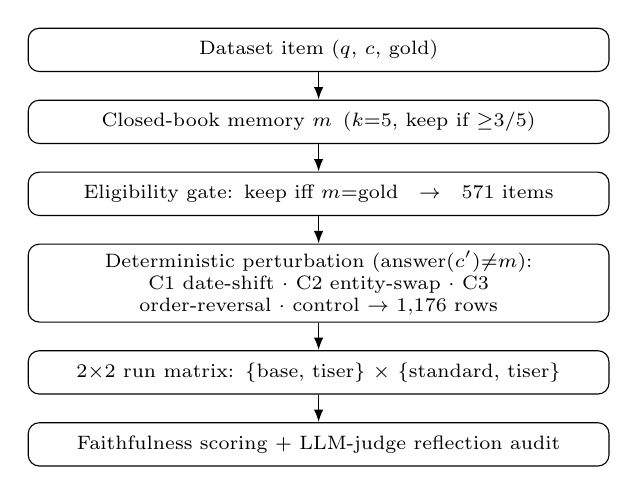
\begin{tikzpicture}[
  node distance=3.5mm,
  box/.style={draw, rounded corners, align=center, font=\scriptsize, text width=72mm, inner sep=2.5pt, minimum height=5.5mm},
  arr/.style={-{Latex[length=1.6mm]}, semithick}
]
\node[box] (n1) {Dataset item $(q,\,c,\,\text{gold})$};
\node[box, below=of n1] (n2) {Closed-book memory $m$\, ($k{=}5$, keep if ${\geq}3/5$)};
\node[box, below=of n2] (n3) {Eligibility gate: keep iff $m{=}\text{gold}\ \rightarrow\ 571$ items};
\node[box, below=of n3] (n4) {Deterministic perturbation ($\text{answer}(c'){\neq}m$): C1 date-shift $\cdot$ C2 entity-swap $\cdot$ C3 order-reversal $\cdot$ control $\rightarrow$ 1{,}176 rows};
\node[box, below=of n4] (n5) {$2{\times}2$ run matrix: \{base, tiser\} $\times$ \{standard, tiser\}};
\node[box, below=of n5] (n6) {Faithfulness scoring\ $+$\ LLM-judge reflection audit};
\draw[arr] (n1)--(n2);
\draw[arr] (n2)--(n3);
\draw[arr] (n3)--(n4);
\draw[arr] (n4)--(n5);
\draw[arr] (n5)--(n6);
\end{tikzpicture}
\caption{The inference-only Context--Memory Conflict pipeline: closed-book memory elicitation, an eligibility gate that keeps only confidently-recalled facts, deterministic counterfactual perturbation into conflict classes, a $2{\times}2$ model$\times$prompt run matrix, and faithfulness scoring plus an LLM-judge reflection audit.}
\label{fig:pipeline}
\end{figure}

\subsection{Tennis Domain Adaptation for Temporal Reasoning}

The second extension is a tennis-domain adaptation study. It first evaluates lightweight 0.5B tennis-only LoRA adaptation on professional-tennis narratives, then evaluates 7B transfer from the original TISER adapter and continued tennis adaptation initialized from that adapter. Mixed tennis+TISER replay and original-TISER forgetting evaluation are left outside the reported result set.

\section{Methodology}
\label{sec:methodology}

\subsection{Baseline TISER Reproduction}

TISER decomposes temporal reasoning into four stages~\cite{bazaga2025tiser}: reasoning, timeline construction, reflection, and answer generation, all produced autoregressively in a single pass. The target supervision format teaches the model to externalize temporal structure before answering.

We use the Amazon-released TISER JSONL data. After a 2,048-token length filter, the training set contains 54,488 examples. The test set contains 22,014 examples (19,214 in-domain, 2,800 OOD ToT-semantic).

The base model is \texttt{Qwen2.5-7B-Instruct}, fine-tuned with LoRA~\cite{hu2022lora}: frozen base weights, trainable low-rank adapters on $q$/$k$/$v$/$o$ attention projections, rank $r{=}16$, scaling $\alpha{=}32$, dropout~0.05. Training uses bf16 precision without base quantization, 3 epochs, learning rate $2{\times}10^{-4}$, cosine schedule, warmup ratio~0.03, effective batch size~16, seed~42, and \texttt{paged\_adamw\_8bit}. Each training sample is converted into a Qwen chat-formatted prompt; the instruction/question/context tokens are masked with label $-100$ (completion-only loss). At inference, the model generates the full trace greedily (\texttt{max\_new\_tokens=768}), the \texttt{<answer>} span is extracted by regex, and the prediction is normalized using SQuAD-style normalization before computing Exact Match (EM) and token-level F1.

\paragraph{Setup.}
Fine-tuning ran on a single RunPod H200~SXM GPU (bf16 LoRA, no quantization; $54{,}488{\times}3$ epochs in ${\sim}6.5$\,h, ${\sim}7$ samples/s; seed~42) with PyTorch~2.4.1/CUDA~12.4, Transformers~4.46.3, PEFT~0.13.2 and TRL~0.12.2. Probe inference and the full baseline evaluation run on vLLM~0.22.0 (H100~SXM, bf16, greedy); the remaining CPU stages (subset, eligibility, perturbation, scoring, the reflection-audit join and the analysis) run locally.

\subsection{Extension: Context--Memory Conflict Probe}

The extension is inference-only (no new fine-tuning); the subject model is the frozen \texttt{Qwen2.5-7B-Instruct} + TISER adapter. Fig.~\ref{fig:pipeline} summarises the pipeline.

\paragraph{Subset, memory, eligibility (M0--M2).}
We keep the in-scope real-entity splits (TempReason L2/L3, TimeQA easy/hard; 15,898 items); TGQA is excluded as its synthetic/fictional entities lack the parametric belief needed for a knowledge-conflict probe. For each item the temporal context is deleted and the closed-book answer $m$ is elicited from $k{=}5$ samples at $T{\approx}0.7$, keeping the majority if it appears in ${\geq}3/5$ samples. An item is \emph{eligible} iff $m$ is confident and equals the original gold answer, ensuring a genuine memorised belief; this yields 571 eligible items.

\paragraph{Deterministic perturbation (M3).}
Each eligible item is edited into conflict classes:
\textbf{C1 (date-shift)} moves date ranges so a different entity covers the queried time-point;
\textbf{C2 (entity-swap)} replaces the answer entity with a same-type distractor;
\textbf{C3 (order-reversal)} swaps intervals so a before/after relation flips.
A \emph{control} arm reorders rows without changing the answer. Each edit enforces the invariant $\text{answer}(c'){\neq}m$, yielding 1,176 rows (C1 203, C2 520, C3 333, control 120) at 100\% per-class construction validity.

\paragraph{Run matrix (M4--M5).}
We cross \emph{model}~$\in$~\{vanilla Qwen (\texttt{base}), TISER fine-tuned (\texttt{tiser})\} with \emph{prompt}~$\in$~\{standard direct-answer, TISER 4-tag prompt\}; only TISER-prompt cells produce a \texttt{<reflection>} trace.

\paragraph{Scoring and reflection audit (M6--M7).}
M6 scores each prediction for faithful-EM/F1 (matches $\text{answer}(c')$), memorised-EM (matches $m$) and malformed rate. M7 is a separate post-hoc \emph{LLM-judge reflection audit}: a Claude-based evaluator reads each \texttt{<reflection>} from the TISER-prompt cells and returns a structured verdict---\texttt{conflict\_raised} (bool), \texttt{conflict\_kind} $\in$ \{\texttt{timeline\_inconsistency}, \texttt{context\_error}, \texttt{context\_vs\_answer}\}, and a short rationale---processed in windows of 100 reflections. The audit labels persisted traces and does not regenerate model answers; it replaces a first-pass lexical mention proxy.

\subsection{Tennis Adaptation Dataset and Method}

The raw tennis set contains 1,122 temporal QA examples covering before/after relations, first/last events, immediate order, durations, overlap, tournament rounds, and medical timing. Audit and conversion add ids, rule-based categories, prompts, and TISER-compatible fields; duplicate-aware splitting with seed~42 yields 785 train, 113 dev, and 224 test examples.

The tennis evaluator keeps the TISER parser and completion format---\texttt{<reasoning>}, \texttt{<timeline>}, \texttt{<reflection>}, \texttt{<answer>}---and adds tennis-specific answer normalization for rankings, minute durations, punctuation, and articles. In addition to base \texttt{Qwen2.5-0.5B-Instruct} standard/TISER-prompt runs, we trained and evaluated a lightweight tennis-only LoRA adapter in the \texttt{full600} condition. We also evaluated \texttt{Qwen2.5-7B-Instruct} with the original TISER adapter on the same tennis test set, then ran continued tennis-from-TISER LoRA experiments initialized from that adapter. Mixed tennis+TISER replay and original-TISER forgetting evaluation are excluded from the reported result set.

\section{Experiments and Results}

\subsection{Baseline Reproduction}

Table~\ref{tab:baseline} reports our full in-domain test results. Our reproduction achieves macro-EM~0.878 / macro-F1~0.949 across the five in-domain splits. The original paper reports Qwen2.5-7B + TISER at macro-EM~0.911 / macro-F1~0.944 for the comparable in-domain configuration. Our result is in the same performance regime; remaining differences may stem from training infrastructure, data preprocessing, or stochastic variation.

\begin{table}[t]
\centering
\caption{Baseline reproduction on the full in-domain test set, against the paper's Qwen2.5-7B + TISER numbers. Macro is over the five in-domain splits; ToT-semantic (OOD, EM~0.381) is excluded.}
\label{tab:baseline}
\setlength{\tabcolsep}{4pt}
{\footnotesize
\begin{tabular}{lrcccc}
\toprule
\textbf{Split} & \textbf{$n$} & \textbf{EM} & \textbf{F1} & \textbf{Paper EM} & \textbf{Paper F1} \\
\midrule
TGQA            & 3{,}316 & 0.571 & 0.870 & 0.845 & 0.942 \\
TempReason L2   & 5{,}397 & 0.907 & 0.929 & 0.855 & 0.875 \\
TempReason L3   & 4{,}426 & 0.961 & 0.974 & 0.915 & 0.949 \\
TimeQA easy     & 2{,}997 & 0.980 & 0.989 & 0.979 & 0.983 \\
TimeQA hard     & 3{,}078 & 0.970 & 0.981 & 0.961 & 0.972 \\
\midrule
\textbf{Macro (5)} & 19{,}214 & \textbf{0.878} & \textbf{0.949} & 0.911 & 0.944 \\
\bottomrule
\end{tabular}
}
\end{table}

TGQA is the only split below the paper on EM (0.571) yet its F1 is high (0.870): inspecting predictions, ${\sim}56\%$ of its well-formed EM$=$0 cases are unit drops (e.g.\ ``8'' vs.\ ``8 years''). Crediting content-correct answers lifts effective TGQA EM to ${\approx}0.85$, matching the paper's 0.845, so the macro-EM gap is largely an exact-match formatting artifact rather than a reasoning gap.

\subsection{Context--Memory Conflict: Run Matrix}

Table~\ref{tab:conflict} reports faithfulness and memorisation rates across all four cells of the run matrix ($n{=}1{,}176$ conflict rows per cell).

\begin{table}[t]
\centering
\caption{Context--Memory Conflict run matrix. All metrics are rates over $n{=}1{,}176$ counterfactual items. The \emph{refl-conflict} column is the LLM-judge reflection audit, reported only for TISER-prompt cells.}
\label{tab:conflict}
\setlength{\tabcolsep}{3pt}
\begin{tabular}{llccccc}
\toprule
\textbf{Model} & \textbf{Prompt} & \textbf{faith-EM} & \textbf{faith-F1} & \textbf{mem-EM} & \textbf{malf.} & \textbf{refl-conf.} \\
\midrule
tiser  & tiser    & \textbf{0.787} & \textbf{0.917} & 0.230 & 0.002 & 0.042 \\
tiser  & standard & 0.574 & 0.771 & 0.297 & 0.000 & ---   \\
base   & tiser    & 0.561 & 0.739 & 0.295 & 0.003 & 0.074 \\
base   & standard & 0.380 & 0.605 & 0.332 & 0.000 & ---   \\
\bottomrule
\end{tabular}
\end{table}

The TISER prompt raises faithful-EM by $+0.213$ ($95\%$ CI $[+0.187,+0.238]$) on the fine-tuned model (0.787 vs.\ 0.574). Fine-tuning raises faithful-EM by $+0.225$ ($[+0.196,+0.256]$) under the TISER prompt (0.787 vs.\ 0.561). Both axes contribute substantially. Item-level bootstrap $95\%$ CIs (2{,}000 resamples) on the four cells are $[.764,.810]$, $[.545,.602]$, $[.532,.590]$ and $[.352,.409]$, and both head-line gaps are significant under a paired McNemar test (prompt axis $\chi^2{=}219.9$; model axis $\chi^2{=}189.9$; both $p{<}10^{-40}$, $n{=}1{,}176$). The base model names conflicts in its reflection more often than the TISER fine-tune (7.4\% vs.\ 4.2\%, LLM-judge audit) yet is less faithful, so naming a conflict is not the same as resolving it. Fig.~\ref{fig:results} visualises both axes and the per-class breakdown.

\begin{figure}[t]
\centering
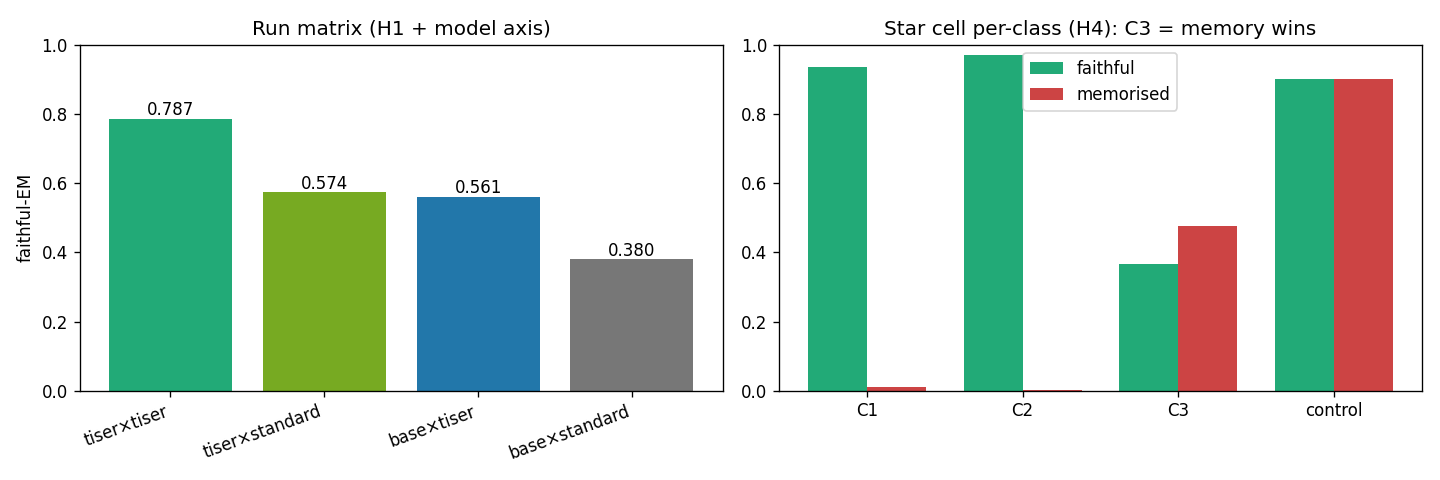
\includegraphics[width=\columnwidth]{figures/conflict_summary.png}
\caption{Left: faithful-EM across the $2{\times}2$ run matrix (the H1 prompt axis and the model/SFT axis). Right: per-class faithful vs.\ memorised EM for the star cell (tiser$\times$tiser); the C3 order-reversal bar is the only class where memory overtakes the text (H3).}
\label{fig:results}
\end{figure}

\subsection{Per-Conflict-Class Results (Star Cell)}

Table~\ref{tab:perclass} breaks down the star cell (\texttt{tiser}$\times$\texttt{tiser}) by conflict type.

\begin{table}[t]
\centering
\caption{Per-conflict-class results for the star cell (tiser$\times$tiser). \emph{judge-refl} is the LLM-judge conflict-naming rate. For \emph{control}, $\text{answer}(c'){\equiv}m$ by construction, so faithful- and memorised-EM coincide.}
\label{tab:perclass}
\setlength{\tabcolsep}{4pt}
{\footnotesize
\begin{tabular}{lrcccl}
\toprule
\textbf{Class} & \textbf{$n$} & \textbf{faith-EM} & \textbf{mem-EM} & \textbf{judge-refl} & \textbf{Reading} \\
\midrule
C1 date-shift      & 203 & 0.936 & 0.010 & 0.020 & follows text \\
C2 entity-swap     & 520 & 0.971 & 0.002 & 0.008 & follows text \\
C3 order-reversal  & 333 & 0.366 & 0.477 & 0.111 & memory wins  \\
control            & 120 & 0.900 & 0.900 & 0.033 & sanity floor \\
\bottomrule
\end{tabular}
}
\end{table}

C1 (date-shift) and C2 (entity-swap) are largely solved: the fine-tuned model reliably follows the edited text (faithful-EM~${\geq}0.936$). C3 (order-reversal) is the blind spot, where faithfulness collapses to 0.366 and memorised answers overtake faithful ones (0.477 vs.\ 0.366). The audit ties H2 to H3: the model raises the clash almost only on C3 (11.1\%, vs.\ ${\leq}2\%$ on C1/C2)---it tends to notice exactly the class it fails. The control arm is a sanity floor, not a faithfulness contest: because $\text{answer}(c'){\equiv}m$ by construction, its faithful- and memorised-EM coincide (0.900), measuring only whether a benign edit preserved answerability. Control is also a different, L3-heavy subsample (58\% TempReason-L3) and is not prompt-independent---the same items score only 0.700 under the standard prompt---so its 0.900 is not proof that the edits are universally clean.

\subsection{Tennis Domain Adaptation Results}

Table~\ref{tab:tennis-final} reports the completed 0.5B 224-example tennis-test runs. We do not treat smaller smoke conditions as final test results.

\begin{table}[t]
\centering
\caption{Tennis temporal QA results on the 224-example test set with Qwen2.5-0.5B-Instruct. Deltas are computed against the base standard prompt.}
\label{tab:tennis-final}
\setlength{\tabcolsep}{3pt}
{\footnotesize
\begin{tabular}{lccccc}
\toprule
Condition & EM & F1 & $\Delta$EM & $\Delta$F1 & Malf. \\
\midrule
Base standard & 0.379 & 0.472 & -- & -- & 0 \\
Base + TISER prompt & 0.375 & 0.420 & -0.004 & -0.052 & 5 \\
Tennis-only adapter & 0.464 & 0.516 & +0.085 & +0.045 & 0 \\
\bottomrule
\end{tabular}
}
\end{table}

Table~\ref{tab:tennis-7b} reports the completed 7B tennis transfer and continued-adaptation runs. Deltas are computed against direct transfer of the original TISER adapter to the tennis test set.

\begin{table}[t]
\centering
\caption{Qwen2.5-7B tennis-transfer and continued-adaptation results on the 224-example tennis test set.}
\label{tab:tennis-7b}
\setlength{\tabcolsep}{3pt}
{\footnotesize
\begin{tabular}{lccccc}
\toprule
Condition & EM & F1 & $\Delta$EM & $\Delta$F1 & Malf. \\
\midrule
Original TISER transfer & 0.580 & 0.701 & -- & -- & 0 \\
Best tennis-from-TISER & 0.732 & 0.856 & +0.152 & +0.155 & 0 \\
\bottomrule
\end{tabular}
}
\end{table}

The \texttt{tennis\_only\_trace50\_smoke\_100} run is kept only as a 100-example smoke check (EM~0.330, F1~0.377, one malformed output), not as the main tennis-test result.

\section{Analysis}

\subsection{Baseline}

Our reproduction reaches the same general performance regime as the original TISER paper. EM is brittle for free-form temporal QA, especially when answers differ only by units, punctuation, or symmetric phrasing (the TGQA case above); token-F1 and qualitative inspection are useful complements.

\subsection{Extension}

\textbf{H1 (context-faithfulness) is supported.} Both the TISER prompt and TISER fine-tuning independently increase context-faithfulness under conflict. The combined effect raises faithful-EM from the base-standard floor of 0.380 to 0.787.

\textbf{H2 reveals silent override.} The TISER fine-tuned model often follows the edited context (78.7\%) but almost never explicitly notices that the context contradicts its memorised belief: an LLM-judge audit of all 1,176 reflections puts the conflict-naming rate at 4.2\%, barely above the 2.3\% baseline revise-rate measured on normal (non-conflict) data. This rare noticing is driven by conflict \emph{type}, not memory strength---it concentrates on C3, is non-monotonic in the closed-book self-consistency score (peaking at 4/5 rather than 5/5), and even when a clash is flagged the answer still reverts to memory in 23 of the 49 flagged star-cell rows. TISER turns Qwen into a grounded reader, but not a genuine auditor.

\textbf{H3 (conflict-type dependence) is supported.} Date-shift and entity-swap conflicts are nearly solved (faithful-EM $\geq$~0.936), while order-reversal causes a collapse in faithfulness where the model reverts to its memorised event ordering. This is the only conflict class where memorised-EM exceeds faithful-EM.

\subsection{Tennis-Domain Status}

TISER prompting alone does not improve the small base model on the full tennis test set: EM changes from 0.379 to 0.375 and F1 drops from 0.472 to 0.420, with five malformed outputs. The tennis-only \texttt{full600} LoRA adapter improves over the standard base prompt by +0.085 EM and +0.045 F1. In the 7B setting, the original TISER adapter transfers to tennis at EM~0.580 / F1~0.701, and continued tennis-from-TISER adaptation improves this to EM~0.732 / F1~0.856. These results support a domain-adaptation gain beyond the lightweight 0.5B result. Mixed replay and original-TISER forgetting are excluded from the reported result set, so preservation of general TISER performance is not evaluated.

\subsection{Caveats}

Conflict-naming is decided by a single automated LLM judge; it agrees with the discarded keyword proxy only moderately (Cohen's $\kappa{=}0.76$ on the star cell), and no second independent judge or human-calibration round has been run. The eligible set is biased toward facts the model already knows confidently, so 0.787 faithful-EM characterises performance on strong memory conflicts, not a random sample of all temporal QA. All cell scores are single greedy decodes, though we report item-level bootstrap CIs and paired McNemar tests for the headline comparisons. Finally, the reflection text should not be interpreted as mechanistically faithful reasoning.

\section{Conclusions}

Our reproduction of TISER under a single-GPU LoRA setup succeeds, reaching macro-EM~0.878 / macro-F1~0.949 on the full in-domain test set. TISER's structured trace (reasoning, timeline, reflection, answer) improves temporal QA performance.

The Context--Memory Conflict extension shows that TISER substantially improves context-faithfulness under counterfactual contexts: faithful-EM rises from 0.380 (vanilla baseline) to 0.787 (TISER fine-tune + TISER prompt). However, the reflection stage usually accepts the generated answer rather than explicitly detecting contradictions between the context and memorised knowledge (4.2\% conflict-naming rate by the LLM-judge audit vs.\ a 2.3\% baseline revise-rate). Event-ordering conflicts (C3) remain a weakness where the model reverts to memorised temporal order despite contradictory context.

For the tennis extension, lightweight tennis-only adaptation produces a small but measurable gain on the 224-example tennis test set (EM 0.379 to 0.464). The completed 7B tennis-from-TISER experiments improve over direct original-TISER transfer from EM~0.580 / F1~0.701 to EM~0.732 / F1~0.856. Mixed tennis+TISER replay and forgetting on the original TISER sample are excluded from the reported result set.

\section{Reproducibility}

The pipeline is config-driven (\texttt{config/config.yaml}, \texttt{config/conflict.yaml}) with fixed seed~42. Each baseline and extension run saves \texttt{run\_meta.json} recording the git SHA, library versions, and resolved configuration. Predictions and per-example EM/F1 scores are saved for error analysis. Extension artifacts are organized under \texttt{outputs/conflict/<stage>/}; each pipeline stage (M0 subset, M1 memory, M2 eligibility, M3 conflicts, M4 prompts, M5 generations, M6 scoring, M7 reflection audit, M10 analysis) writes a JSON/JSONL artifact and its own \texttt{run\_meta.json}. Source code and this report are in the project repository at \href{https://github.com/thestbobo/tiser_temporal_reasoning_extension}{GitHub repository}.

\begin{thebibliography}{00}

\bibitem{bazaga2025tiser}
A. Bazaga, R. Blloshmi, B. Byrne, and A. de Gispert,
``Learning to Reason Over Time: Timeline Self-Reflection for Improved Temporal Reasoning in Language Models,''
in \emph{Proceedings of ACL}, 2025.

\bibitem{xiong2024tgqa}
S. Xiong, A. Payani, R. Kompella, and F. Fekri,
``Large Language Models Can Learn Temporal Reasoning,''
in \emph{Proceedings of ACL}, 2024.

\bibitem{tan2023tempreason}
Q. Tan, H. T. Ng, and L. Bing,
``Towards Benchmarking and Improving the Temporal Reasoning Capability of Large Language Models,''
in \emph{Proceedings of ACL}, 2023.

\bibitem{chen2021timeqa}
W. Chen, X. Wang, and W. Y. Wang,
``A Dataset for Answering Time-Sensitive Questions,''
in \emph{NeurIPS Datasets and Benchmarks}, 2021.

\bibitem{hu2022lora}
E. J. Hu et al.,
``LoRA: Low-Rank Adaptation of Large Language Models,''
in \emph{International Conference on Learning Representations}, 2022.

\end{thebibliography}

\end{document}
